\chapter{Annotation Service}

\section{Objective of the Annotation Service}
As described in 2.4.2, the goal of the AS is to provide a user with the possibility to:
\begin{enumerate}[(1)]
	\item view A WSI
	\item annotate a WSI
	\item manage made annotations
\end{enumerate}

In order to achieve objective (1) - (3), a GUI needs to be deployed which supports the user in working on those tasks. (3) also adds the need for file persistence management.


\section{Methodology}
As stated in 2.1, most vendors have proprietary image formats and their own implementation of a viewer for those, thus creating a vendor lock-in. Further do vendors often only support Windows platforms, ignoring other operating systems\cite{Cornish13}\cite{DICOM10}\cite{Farahanil15}. To avoid this, a solution must be found that is independent of operating system and vendor.

Chap. 3 already established a service to convert WSIs of various formats into the DZI format, solving the problem of multiple proprietary formats. 

Independence from an operating system can be achieved by using web technologies, especially when running an application in a web browser\cite{Tseytlin14}, since those are supported by all modern operating systems. 

Because of this, the AS will be implemented as a web browser application. 


\subsection{Parts of the Annotation Service}
The AS is implemented in 2 parts. These are the Annotation Service Server (ASS)\nmc{ASS}{Annoation Service Server} and the Annotation Service Viewer (ASV)\nmc{ASV}{Annotation Service Viewer}.

This is because of the \emph{same-origin policy} (SOP)\nmc{SOP}{same-origin policy}. SOP is a security concept of the web application security model. It prevents a direct access to files, if the parent directory of the originating file is not an ancestor directory of the target file\cite{web:mdn}. Because of the SOP, WSIs would have to be located in the directory structure of the AS, which by itself doesn't create a problem. To get a new WSI there, however, the user would be forced to navigate through the structure of the AS, find the correct directory and then place a the WSI there manually. This makes knowledge of the service structure necessary and creates a horrible UX. Furthermore, tinkering with the file structure of the AS creates a possible error source.

A workaround of this problem is to deploy a web server, which can redirect the image request, access the WSI and return it in response\cite{Tseytlin14}. The use of DZI creates another advantage here. The used image pyramid model reduces the network traffic necessary to load and show a WSI in a viewer\cite{Cornish13}\cite{DICOM10}.

Furthermore, even a single WSI takes up a lot of storage capacity\cite{Singh11}. Having multiple on a local storage would either create the need for huge amounts of available storage space or restrict the amount of accessible WSIs to a few at any given time. The latter solution would create two follow-up problems:
\begin{itemize}
	\item WSIs are medical images and as such confidential information. Therefore, not everyone is allowed to just have access to or copies of a WSI\cite{COA}\cite{USSanDiego}. URLs are easier to manage, since they access one centralized resource, making it easier to regulate access. Once a copy of a WSI changes hands, it is virtually impossible to make sure that privacy regulations are uphold.
	\item With only a subset of all WSIs present at all times, the work of the user is impacted and slowed down greatly. It becomes necessary to make sure to have all WSIs of the current set in a completely annotated state without any errors, before switching to the next set, because the process of copying WSIs back and forth is time consuming. Correcting errors, as well as adding, updating and changing annotations will probably also involve the need to go over most or all WSIs the user has access to. Not only is this slow and inefficient, it also creates a new source for possible errors and mistakes.
\end{itemize}

With the use of a web server as a central image repository, WSIs and the access to them can easily be managed in a centralized spot, while upholding confidentiality regulations. Furthermore, a user has access to all his WSIs at any given time, without the need for subsets or copying files back and forth.

Depending on the setup of the network, other factors can come into play as well, such as access to and sharing of rare cases, educational material, training samples and consulting experts independent of their physical position on the planet\cite{Wilbur09}.


\subsubsection{Annotation Service Server}
% web browser needs server to deliver images
% local for now


\subsubsection{Annotation Service Viewer}
To enable the pathologist to view a WSI and make annotations, a GUI needs to be deployed. This GUI will be called Annotation Service Viewer and developed in an iterative approach with the help of selected pathologists. After each iteration, they'll evaluate the GUI and user experience (UX)\nmc{UX}{User Experience} of the ASV and give feedback. This way, the ASV can be adapted to the needs of a real life environment based on the pathologists feedback.

\begin{figure}[H]
	\begin{center}
		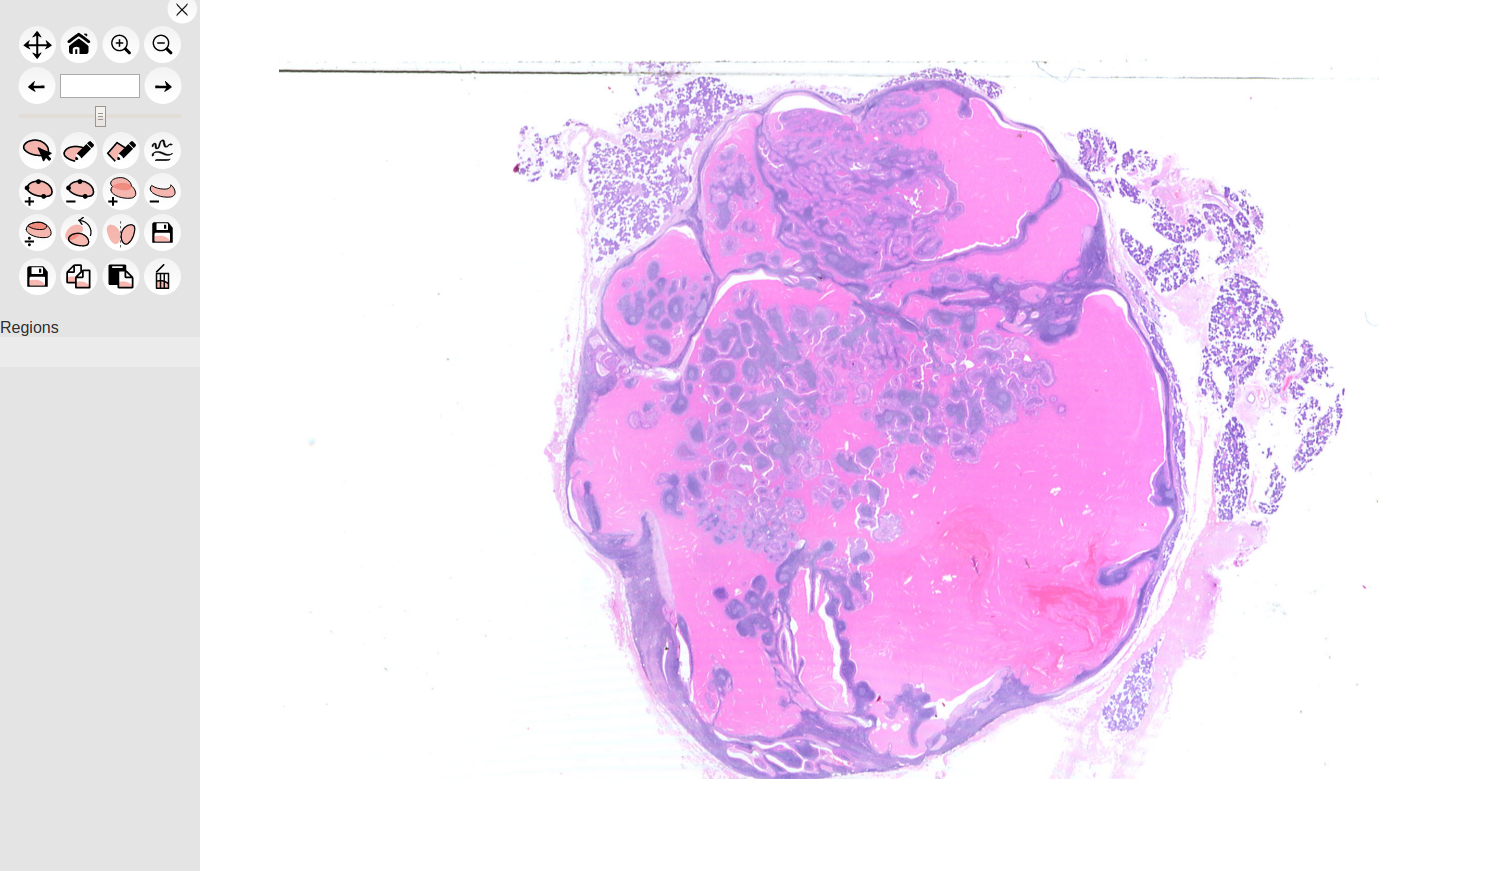
\includegraphics[scale=0.2]{img/microdrawUI.png}
		\caption{Microdraw GUI with opened WSI}
		\label{fig4_microdrawUI}
	\end{center}
\end{figure}

The first iteration of the AS will be based on Microdraw\footnote{See \url{https://github.com/r03ert0/microdraw} for more information on the Microdraw project} (see fig. \ref{fig4_microdrawUI} for it's GUI). Microdraw is a web application, which describes itself as

\begin{quotation}
	"[...] a collaborative vectorial annotation tool for ultra high resolution data, such as that produced by high-throughput histology." \cite{web:microdraw}
\end{quotation}

will run as a web application in a browser. Annotations will be made by selecting a shape or annotation method from the various tools in the toolbar (see the gray bar on the left in fig. 2.5). After selecting the area to be annotated, an actual description of that area can be made via keyboard input.


\subsection{Functionality}
% shortcuts, funtions, etc. pp.

\section{Implementation}
% what was used for implementation
\subsection{Technologies and Frameworks}
% openslide, openslide web server
% python web server, flask, openslide, java script, html5, css
\subsection{Annotation Service Viewer}
% documentation
\subsection{Annotation Service Server}
% documentation